\documentclass[../physics12.tex]{subfiles}
\graphicspath{{\subfix{../figures/}}}
\begin{document}
\chapter{Capacitors and DC Circuits}
\section{Formulas}
Definition of capacitance: $C=Q/V$

Energy stored in a capacitor: 
\[ U = \frac{Q^2}{2C}=\frac{1}{2}CV^2 = \frac{1}{2}QV \]

Parallel plate capacitance w/o dielectric: $C = \epsilon_0 A/d$

Parallel plate capacitance w/ dielectric: $C = \kappa \epsilon_0 A/d$

Capacitors in series: $\frac{1}{C} = \frac{1}{C_1}+\frac{1}{C_2}+\dots + \frac{1}{C_n}$

Capacitors in parallel: $C=C_1+C_2+\dots+C_n$

Definition of current: $i=\Delta Q/\Delta t$

Current and drift velocity: $I=nqv_d A$

Definition of resistance: $R=\Delta V/I$

Resistance of a wire: $R=\rho l/A$

Temperature variation of resistivity: 
\[ \rho = \rho_0 [1+\alpha(T-T_0)] \]

Power dissipation in a resistor:
\[ P = I\Delta V = I^2 R = \frac{\Delta V^2}{R} \]

Steps: in application of Kirchhoff's Rules 
\begin{itemize}
    \item Label current: $i_1,i_2,i_3,\dots$
    \item Node equation: $\sum i_{\text{in}} = \sum i_{\text{out}}$
    \item Loop equation: $\sum (\pm V) + \sum{\mp iR} = 0$
\end{itemize}

Resistors in series: $R = R_1+R_2+\dots+R_n$

Resistors in parallel: $\frac{1}{R}=\frac{1}{R_1}+\frac{1}{R_2}+\dots + \frac{1}{R_n}$

Charging in an RC circuit: $q(t) = Q(1-e^{-t/RC})$

Discharging in an RC circuit: $q(t) = Qe^{-t/RC}$, where RC = $\tau$ is the time constant.

\section{Electrons Through a Resistor Problem}
If $5\times 10^{21}$ electrons pass through a $20\Omega$ resistor in 10 min, what is the potential difference across the resistor? 
The fundamental charge is $1.602\times 10^{-19}$ C. Answer in units of V.

\section{Voltage across a capacitor problem}
Consider the capacitor network
\begin{center}
    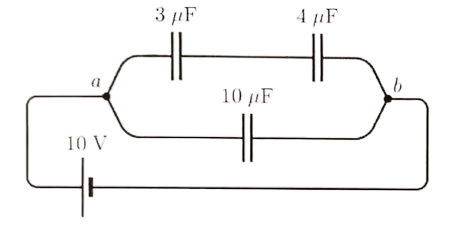
\includegraphics[width=0.5\textwidth]{10.2.PNG}
\end{center}
What is the voltage across the 4 $\mu$F (upper right hand) capacitor? Answer in units of V.

\section{Unknown Capacitance Problem}
When the switch is in position a, an isolated capacitor of unknown capacitance has been charged to a potential difference of 100 V. When the switch 
is moved to position b, this charged capacitor is then connected parallel to the uncharged 10 $\mu$F capacitor. The voltage across the combination becomes 30 V.
\begin{center}
    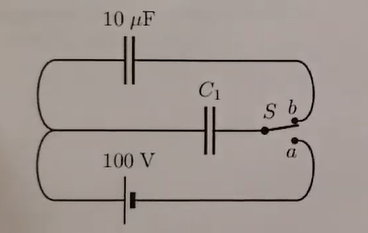
\includegraphics[width=0.5\textwidth]{10.3.PNG}
\end{center}
Calculate the unknown capacitance. Answer in units of $\mu$F.

\section{Drift Velocity Problem}
An aluminum wire with a cross-sectional area of $4\times 10^{-6}$ m$^2$ carries a current of 5 A. 

Find the drift speed of the electrons in the wire. Assume that each atom supplies one electron. Aluminum has a molecular weight of 26.98 g/mol and a density of 
2.7 g/cm$^3$. Avogadro's number is $6.022\times 10^{23}$ and the fundamental charge is $1.602\times 10^{-19}$ C. Answer in units of m/s.

\section{Equivalent Resistance Problem}
Four resistors are connected as shown in the figure.
\begin{center}
    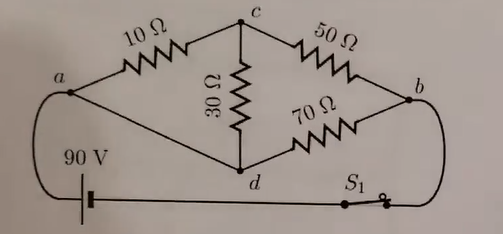
\includegraphics[width=0.5\textwidth]{10.5.PNG}
\end{center}
Find the resistance between points $a$ and $b$. Answer in units of $\Omega$.

\section{Find R in Circuit with Switch Problem}
In the circuit shown below, the current $i$ in the resistor $R$ doubles its original value when the switch $S$ is closed.
\begin{center}
    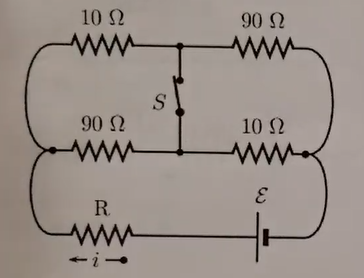
\includegraphics[width=0.5\textwidth]{10.6.PNG}
\end{center}
Find the value of $R$. Answer in units of $\Omega$.

\section{Charge on Capacitor Problem}
In the figure below the battery has an emf of 4 V and an internal resistance of $1 \Omega$. Assume there is a steady current flowing in the circuit.
\begin{center}
    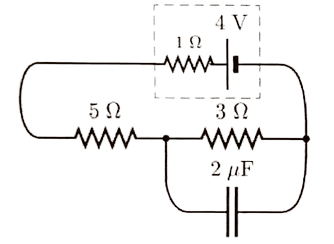
\includegraphics[width=0.5\textwidth]{10.7.PNG}
\end{center}
Find the charge on the 2 $\mu$F capacitor. Answer in units of $\mu$C.

\section{Voltage across Capacitor Problem}
The circuit has been connected as shown in the figure for a ``long'' time. 
\begin{center}
    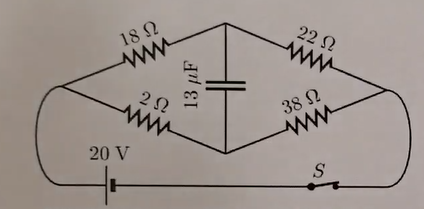
\includegraphics[width=0.5\textwidth]{10.8.PNG}
\end{center}
What is the magnitude of the electric potential across the capacitor? Answer in units of V.

\section{Two Loop Circuit Problem}
Consider the circuit
\begin{center}
    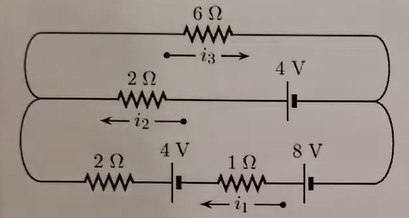
\includegraphics[width=0.5\textwidth]{10.9.PNG}
\end{center}

Find $i_1$. Answer in units of A.

\end{document}